\chapter{Livello IP}
\section{Importanza e compiti del livello Netwrok}
Viene definita l'unità di trasferimento dati, ossia il Datagramm (da 64 a 1500 byte). Inoltre, garantisce l'indirizzamento univoco degli host, infatti, tutti gli host connessi a Internet devono essere identificati tramite un Indirizzo IP anche grazie al fatto che viene chiarita l'architettura di Internet. Tutti i router e i sistemi autonomi che compongono Internet possono essere raggiunti tramite funzioni di routing, ossia algoritmi  determinano il percorso dei dati all'interno di una rete geografica. La consegna dei datagrammi però non è affidabile (best-effort).

\begin{figure}[!htb]
    \centering
    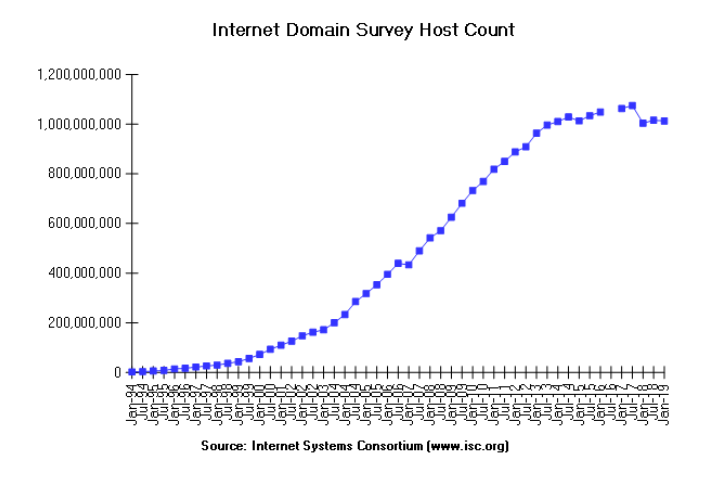
\includegraphics[width=0.7\linewidth]{Images/livello_ip/NumeroIPV4.png}
    \caption{Grafico degli IPv4 unovici su Internet.}
\end{figure}

Non tutti i protocolli a livello Network forniscono un sistema di consegna non affidabile, per esempio la telefonia fornisce un approccio \textbf{connection-oriented}, rispetto all'approccio \textbf{connection-less} di Internet.
Infatti:
\begin{itemize}
    \item \textbf{Circuit Switching:} è necessario riservare tutte le risorse end-to-end prima della trasmissione:
    \begin{itemize}
        \item Non è possibile condividere le risorse assegnate.
        \item Per ogni chiamata è necessaria una fase di configurazione.
        \item Prestazioni garantite in base al tipo di risorse riservate.
    \end{itemize}
    \item \textbf{Packet Switching:} nessuna risorsa riservata:
    \begin{itemize}
        \item Ogni utente può utilizzare tutte le risorse disponibili.
        \item Nessuna configurazione richiesta.
        \item Rischio di conflitti/congestione.
    \end{itemize}
\end{itemize}



\section{Protocollo IP}

\begin{boxDef}
\textcolor{brown}{Protocollo IP:} è un protocollo di comunicazione a livello netwrok, ideato da Vint Cerf e Bob Kahn nel maggio del 1974 e pubblicato sull'IEEE. La prima versione pubblicata è stato IPv4, il suo successore è IPv6.
\end{boxDef}

Il \textbf{protocollo IP} fornisce alcuni servizi molto importanti:
\begin{itemize}
    \item \textbf{Indirizzamento host univoco:} fornisce un grafico praticamente completo di tutti gli host (indirizzi IP).
    \item \textbf{Unità di trasferimento dati:} definisce l'unità di informazione di base utilizzata da Internet per trasferire dati.
    \item \textbf{Funzioni di Routing:} sceglie il percorso nella rete nel quale inviare i pacchetti.
\end{itemize}
La consegna dei pacchetti, però, non è affidabile:
\begin{itemize}
    \item \textbf{Consegna connectionless:} ogni pacchetto è trattato in modo indipendente rispetto agli altri.
    \item \textbf{Consegna Best-Effort:} tentativo di consegnare ogni pacchetto.
    \item \textbf{Consegna non garantita:} i pacchetti possono essere persi, duplicati, ritardati o consegnati fuori ordine.
\end{itemize}

\subsection{Datagram}
\begin{figure}[!htb]
    \centering
    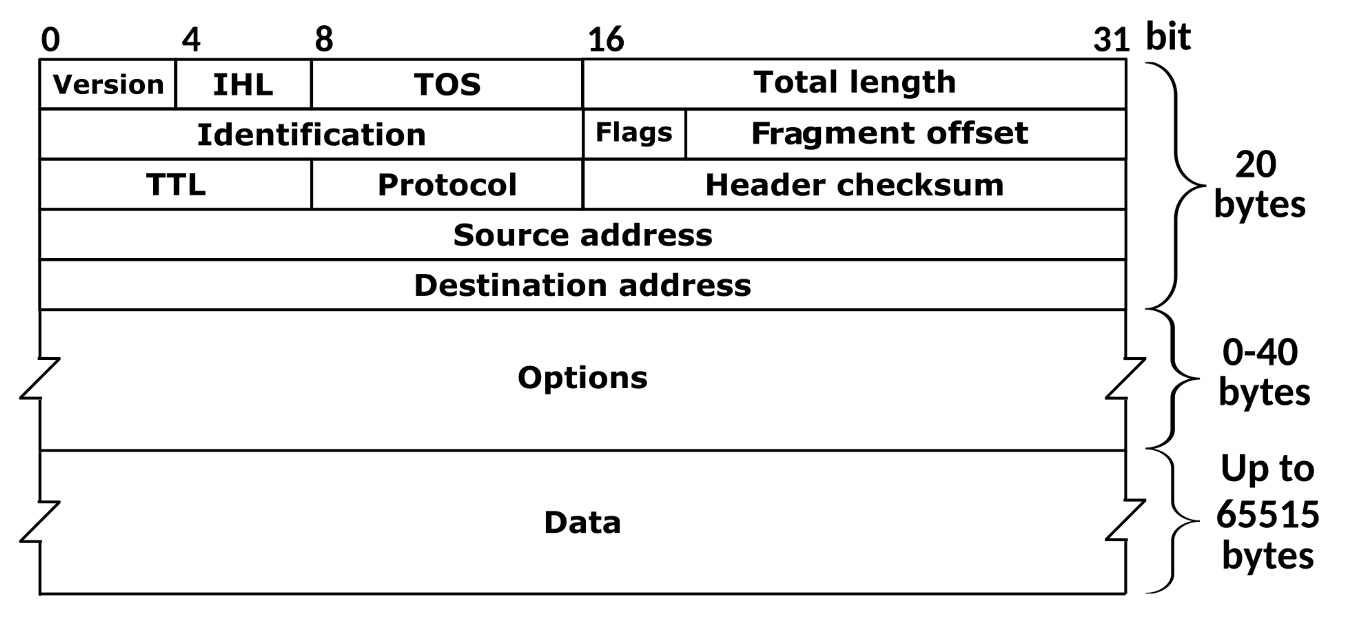
\includegraphics[width=0.9\linewidth]{Images/livello_ip/Datagram.png}
    \caption{Composizione di un Datagram IP.}
\end{figure}

Il \textbf{Datagram IP} è formato da due parti principali, l'header e i dati che effettivamente vengono inviati.
L'header IP a suo volta è formato da diversi campi:
\begin{itemize}
    \item \textbf{Version:} campo da 4 bit con la versione del protocollo IP usato per la creazione del Datagram.
    \item \textbf{IP Header Lenght (IHL):} campo da 4 bit che indica la lunghezza dell'header (massimo 20 byte).
    \item \textbf{Total Lenght:} campo da 16 bit con la lunghezza del Datagram IP (massimo 64kb).
    \item \textbf{Type of Service (TOS):} campo da 8 bit che specifica come il Datagram deve essere trattato, i bit di questo campo sono divisi così:
    \begin{itemize}
        \item \textbf{Precendence:} 3 bit che specificano l'importanza del datagram.
        \item \textbf{Delay (D):} 1 bit.
        \item \textbf{Throughtput (T):} 1 bit.
        \item \textbf{Affidabilità: (R):} 1 bit.
    \end{itemize}
    \item \textbf{Identificazione:} campo da 16 bit che identifica il Datagram.
    \item \textbf{Flags:} controllo della frammentazione:
    \begin{itemize}
        \item \textbf{Reserved.}
        \item \textbf{Don't Fragment (DF).}
        \item \textbf{More Fragment (MF).}
    \end{itemize}
    \item \textbf{Fragment Offset:} indica la posizione del frammento nel datagram originale.
    \item \textbf{Time To Live (TTL):} campo da 8 bit che contiene un contatore (NB: non è un tempo) che indica quanto un datagram può circolare su Internet. Viene decrementato ogni volta che incontra un router e appena arriva a 0 viene eliminato.
    \item \textbf{Protocol:} campo da 8 bit che indica che tipo di protocollo di più alto livello può usare il datagram.
    \item \textbf{Header Checksum:} usato per controllare l'integrità dei dati dell'header del datagram.
    \item \textbf{Indizzo sorgente:} campo da 32 bit con l'indirizzo IP del mandante.
    \item \textbf{Indirizzo di destinazione:} campo da 32 bit con l'indirizzo IP del destinatario.
    \item \textbf{Opzioni:} campo da 32 bit usato per testing e debugging.
    \item \textbf{Padding:} necessario se le opzioni non sono tutte a 32 bit.
\end{itemize}

\section{Ip Addressing}
Ogni indirizzo IPv4 ha 32 bit, diviso in 4 campi da 8 bit ciascuno e seprarati da un punto e sono formati dalla coppia NetID, HostID. Indirizzi nella stessa rete avranno lo stesso NetID ma diverso HostID.

\subsection{Classe di Indirizzi IP}
Per capire quanti bit deve avere il NetID e quanti bit deve avere l'HostID si deve guardare a che classe appartengono:
\begin{itemize}
    \item \textbf{Classe A:} un byte dedicato alla NetID e tre byte dedicati all'HostID. Da 0.0.0.0 a 127.255.255.255.
    \item \textbf{Classe B:} due byte per la NetID e due byte per l'HostID. Da 128.0.0.0 a 191.255.255.255.
    \item \textbf{Classe C:} tre byte per la NetID e un byte per l'HostID. Da 192.0.0.0 a 223.255.255.255.
    \item \textbf{Classe D:} indirizzi multicast riservati. Da 224.0.0.0 a 239.255.255.255. 
    \item \textbf{Classe E:} indirizzi riservati per usi futuri. Da 240.0.0.0 a 255.255.255.254.
\end{itemize}
Ogni IP può essere assegnato dinamicamente o staticammente. Ogni dispositivo può avere più interfacce di rete e quindi avere più IP.
Inoltre, ci sono alcuni indirizzi speciali:
\begin{itemize}
    \item \textbf{Indirizzo della rete:} gli indirizzi con HostID tutto a 0 indicano l'indirizzo della rete.
    \item \textbf{Indirizzo Broadcast:} indirizzi con HostID tutto a 1 funzionano come indirizzo di Broadcast per tutta la rete.
    \item \textbf{Questo Host su questa rete:} l'indirizzo 0.0.0.0 è usato per fare il boot dell'host.
    \item \textbf{Indirizzo di Loopack:} l'indirizzo di classe A con NetID 127 è usato per fare test in locale. Per esempio l'indirizzo Localhost è 127.0.0.1.
\end{itemize}

\section{Subnetting e Supernetting}
La divisione degli indirizzi è molto rigida, per rendere tutto più semplice e maneggevole si possono usare due metodi:
\begin{itemize}
    \item \textbf{Sottoclassi:} per le organizzazioni.
    \item \textbf{Soureclassi:} per gli ISP.
\end{itemize}
Quindi è necessario definire in modo flessibile e logico la coppia \textbf{NetID}, \textbf{HostID}.
Infatti, per definire i bit della NetID viene usata una network mask da 4 byte. Se si fa una operazione di AND fra l'ip e la mask, gli 1 indicheranno la parte dedicata alla NetID e gli 0 indicheranno la parte dedicata all'HostID.

\subsection{Subnetting}
Un'organizzazione può suddividere il proprio spazio di indirizzi host in gruppi chiamati sottoreti:

\begin{figure}[!htb]
    \centering
    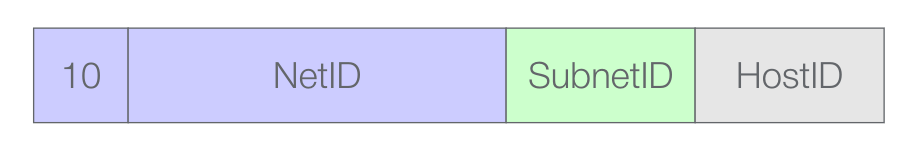
\includegraphics[width=0.7\linewidth]{Images/livello_ip/Subnet.png}
    \caption{Esempio di indirizzo di una subnet.}
\end{figure}

\textbf{ESEMPIO:}
\begin{boxDef}
Dati:
\begin{itemize}
    \item \textbf{IP address:} 192.168.81.56
    \item \textbf{Netmask:} 255.255.255.240
\end{itemize}

Per calcolare il NetID: 
\\
IP Address \textbf{10011100.10011010.01010001.00111000} = \textbf{156.154.81.56}
\\
Netmask \textbf{11111111.11111111.11111111.11110000} = \textbf{255.255.255.240}
\\
Result \textbf{10011100.10011010.01010001.00110000} = \textbf{156.154.81.48}
\end{boxDef}

\section{Architettura di Internet}
Internet non è un insieme di router sparsi a caso per il mondo che sono interconnessi tra loro.
\begin{boxDef}
\textbf{\textcolor{brown}{Internet:}} la definizione di \textbf{Internet} dipende dal punto di vista:
\begin{itemize}
    \item Dal punto di vista delle \textbf{applicazioni di rete}, ossia un'entità trasparente, nella maggior parte dei casi.
    \item Dal punto di vista \textbf{fisico}, un insieme di componenti interni, in cui ogni nodo è caratterizzato da un indirizzo IP.
    \item Dal punto di vista \textbf{organizzativo}, un insieme di sistemi autonomi (considerando i \textbf{router}) e un insieme di nomi e domini (considerando gli \textbf{host}).
\end{itemize}
\end{boxDef}

Ha alcuni principi:
\begin{itemize}
    \item \textbf{Sopravvivenza:} se esiste un percorso tra i due host, la comunicazione deve essere in grado di continuare.
    \item \textbf{Forma a clessidra:} IP fa ipotesi minime sui mezzi di trasferimento dati sottostanti. Deve funzionare per tutti i tipi di applicazioni di rete e con un approccio senza stato.
    \item \textbf{Sistemi autonomi:} ogni rete è di proprietà e gestita da un'entità diversa.
\end{itemize}

\subsection{Autonomous System}
\begin{boxDef}
\textbf{\textcolor{brown}{AS:}} un insieme di \textbf{reti IP} e \textbf{router} sotto il controllo di un'organizzazione all'interno della quale viene utilizzata una politica di \textbf{routing} interna. Tutti i router all'interno dello stesso \textbf{AS} utilizzano lo stesso algoritmo di instradamento dei messaggi e si scambiano continuamente informazioni con gli altri router.
Dall'esterno, i \textbf{sistemi autonomi} sono visti come un'unica entità.
\end{boxDef}
Gli AS sono interconnessi fra di loro in due modi:
\begin{enumerate}
    \item Attraverso punti di peering privati.
    \item Attraverso punti di scambio Internet (IXP).
\end{enumerate}

\section{Routing}
Inoltrare pacchetti all'interno di una rete è un problema complesso, per questo si può dividere in sottoproblemi:
\begin{enumerate}
    \item Ad ogni hop, inoltra il pacchetto a un altro nodo in modo che si avvicini alla destinazione (IP forwarding).
    \item Mantenere le informazioni aggiornate per poter risolvere il primo sottoproblema (Gestione delle tabelle di routing).
\end{enumerate}

\begin{boxDef}
\textbf{\textcolor{brown}{IP Forwarding:}} operazione eseguita da ogni \textbf{router}. Il router successivo deve appartenere alla \textbf{rete} a cui il router è direttamente connesso. Per inoltrare i pacchetti, l'indirizzo di destinazione viene estratto dall'header del \textbf{pacchetto} e viene utilizzato come indice nella tabella di routing.
\end{boxDef}
L'IP forwarding ha alcune caratteristiche importanti:
\begin{itemize}
    \item \textbf{Indipendenza dal mittente:} il routing del next-hop non dipende dal mittente del pacchetto o dal percorso che il pacchetto ha percorso fino a quel punto.
    \item \textbf{Routing universale:} la tabella di routing deve contenere un router next-hop per ogni destinazione.
    \item \textbf{Routing ottimale:} il router next-hop viene scelto in modo da minimizzare il percorso verso la destinazione con l'utilizzo di algoritmi di routing.
\end{itemize}

\begin{boxDef}
\textbf{\textcolor{brown}{Tabelle di Routing:}} ogni host e ogni router possiede una tabella di routing. Ogni riga indica il next-hop per ogni possibile destinazione.
\end{boxDef}

Esistono due tipi di \textbf{Routing}:
\begin{enumerate}
    \item \textbf{Statico:} 
    \begin{itemize}
        \item La tabella di routing non viene modificata dal router.
        \item L'amministratore di rete deve inserire o modificare le righe della tabella di routing.
        \item Impossibilità di reagire automaticamente ai cambiamenti topologici.
        \item Da utilizzare in caso di reti di piccole dimensioni con poche modifiche.
    \end{itemize}
    \item \textbf{Dinamico:}
    \begin{itemize}
        \item La tabella di routing viene modificata dal router al variare delle condizioni di rete.
        \item Lo scambio di informazioni e il calcolo dei valori della tabella di routing avvengono tramite protocolli di routing.
    \end{itemize}
\end{enumerate}

\vspace*{0.02\textheight}
\textbf{ESEMPIO DI IP FORWARDING:}
\begin{figure}[!htb]
    \centering
    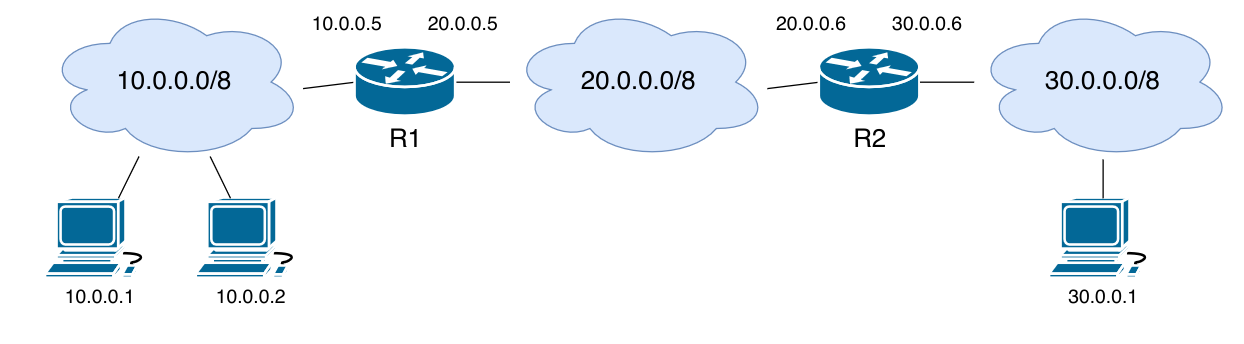
\includegraphics[width=0.8\linewidth]{Images/livello_ip/IPForwarding.png}
    \caption{Esempio di indirizzo di una subnet.}
\end{figure}

Si hanno queste tabelle di routing per quanto riguarda i router:
\begin{center}
    \begin{minipage}{.4\textwidth}
        \begin{tabular}{ || c | c ||}
            \hline
            \textbf{DESTIONATION} & \textbf{NEXT HOP} \\
            \hline
            \hline
            10.0.0.0/8 & direct \\
            \hline
            20.0.0.0/8 & direct \\
            \hline
            30.0.0.0/8 & 20.0.0.6 \\
            \hline
        \end{tabular}
    \end{minipage}
    \begin{minipage}{.4\textwidth}
        \begin{tabular}{ || c | c ||}
            \hline
            \textbf{DESTIONATION} & \textbf{NEXT HOP} \\
            \hline 
            \hline
            10.0.0.0/8 & 20.0.0.5 \\
            \hline
            20.0.0.0/8 & direct \\
            \hline
            30.0.0.0/8 & direct \\
            \hline
        \end{tabular}
    \end{minipage}
\end{center}

E queste tabelle di routing per quanto riguarda gli host:
\begin{center}
    \begin{minipage}{.4\textwidth}
        \begin{tabular}{ || c | c || }
            \hline
            \textbf{DESTIONATION} & \textbf{NEXT HOP} \\
            \hline
            \hline
            10.0.0.0/8 & direct \\
            \hline
            default & 10.0.0.5 \\
            \hline
        \end{tabular}
    \end{minipage}
    \begin{minipage}{.4\textwidth}
        \begin{tabular}{ || c | c || }
            \hline
            \textbf{DESTIONATION} & \textbf{NEXT HOP} \\
            \hline
            \hline
            10.0.0.0/8 & direct \\
            \hline
            default & 30.0.0.6 \\
            \hline
        \end{tabular}
        \label{Tabella di Routing di 30.0.0.1}
    \end{minipage}
\end{center}

\vspace*{0.02\textheight}
Se volessi mandare un pacchetto dall'host \textbf{10.0.0.1} all'host \textbf{10.0.0.2} sarebbe necessario solamente il protocollo ARP, invece, se volessi mandare un pacchetto dallo stesso host sorgente all'host \textbf{30.0.0.1}, dovrei passare prima per il router R1 (sempre tramite il protocollo ARP) e successivamente andare al router R2 per raggiungere l'host di destinazione.

\subsection{Teoria del Routing}
L'obiettivo del routing è stabilire il percorso ottimale, ossia quello con costo minore che colleghi i due host che vogliono comunicare.
Per formulare un algoritmo di routing, la rete viene modellata utilizzando un grafo pesato \textbf{G(N, E)} dove:
\begin{itemize}
    \item I nodi \textbf{N} rappresentano i router (o gli AS).
    \item Gli archi \textbf{E} rappresentano le connessioni tra i router.
    \item Le etichette degli archi \textbf{E} rappresentano il "costo" delle connessioni tra i router.
\end{itemize}
Si dividono in due categorie principali:
\begin{enumerate}
    \item \textbf{Algoritmi di routing distribuiti}:nessun nodo possiede informazioni complete sul costo di tutti i collegamenti nella rete.
    \item \textbf{Algoritmi di routing centralizzati:} ogni nodo possiede informazioni globali sulla rete.
\end{enumerate}

\begin{figure}[!htb]
    \centering
    
\includegraphics[width=0.5\linewidth]{Images/livello_ip/Grafo.png}
    \caption{Grafo pesato.}
\end{figure}

Ci sono alcuni fattori che possono influenzare il routing, come la topologia, traffico, fallimenti e policies.

\newpage
\subsection{Distan Vector Protocol}
Calcolo \textbf{distribuito} del \textbf{next hop}, è un algoritmo adattivo rispetto ai cambiamenti di stato. Esempio di implementazione principale è l'algoritmo distribuito di Bellman-Ford.

\subsubsection{Algortimo di Bellman-Ford}
Compiti di ciascun nodo:
\begin{itemize}
    \item Aggiornamento del vettore di distanza in risposta alle variazioni di costo sui collegamenti adiacenti.
    \item Invio di un aggiornamento ai nodi adiacenti se il loro vettore di distanza cambia.
\end{itemize}
Dati su ciascun nodo \textbf{x}:
\begin{itemize}
    \item $c(x, v)$ costo del collegamento tra il nodo \textbf{x} e il nodo vicino \textbf{v $\in$ V}.
    \item \textbf{Dx} = \{$Dx(y)$ : y $\in$ N\} vettore delle distanze dal nodo x a tutti i nodi \textbf{y} $\in$ rete \textbf{N}.
    \item \textbf{Dv} = \{$Dv(y)$ : y $\in$ N\} vettori di distanza dei nodi vicini \textbf{v} $\in$ \textbf{V} di \textbf{x}.
\end{itemize}
Bellman-Ford serve per calcolare il costo minimo da \textbf{x} a \textbf{y}: 
\[
Dx(y) = min_v\{c(x, v) + Dv(y)\}
\]
Dove $min_v$ è calcolato su tutti i nodi \textbf{v} vicini al nodo \textbf{x}. Tra tutti i nodi \textbf{v} adiacenti al nodo \textbf{x}, il percorso da scegliere è quello che porta da \textbf{v} a \textbf{y} con il costo più basso.

\vspace*{0.02\textheight}
\textbf{INIZALIZZAZIONE:}
\begin{bashbox}
ffor all y in N do
    if y in V then
        Dx(y) = c(x, y)
    else
        Dx(y) = infinito

    Send vector Dx to all v in V
\end{bashbox}

\textbf{LOOP:}
\begin{bashbox}
while True do
    # Wait for change in neighbor link cost or update
    for all y in N do
        Dx(y) = minv{c(x, v) + Dv(y)}
        
        if exist y in N : Dx(y) changed then
            Send vector Dx to all v in V
\end{bashbox}

\begin{figure}[!htb]
    \centering
    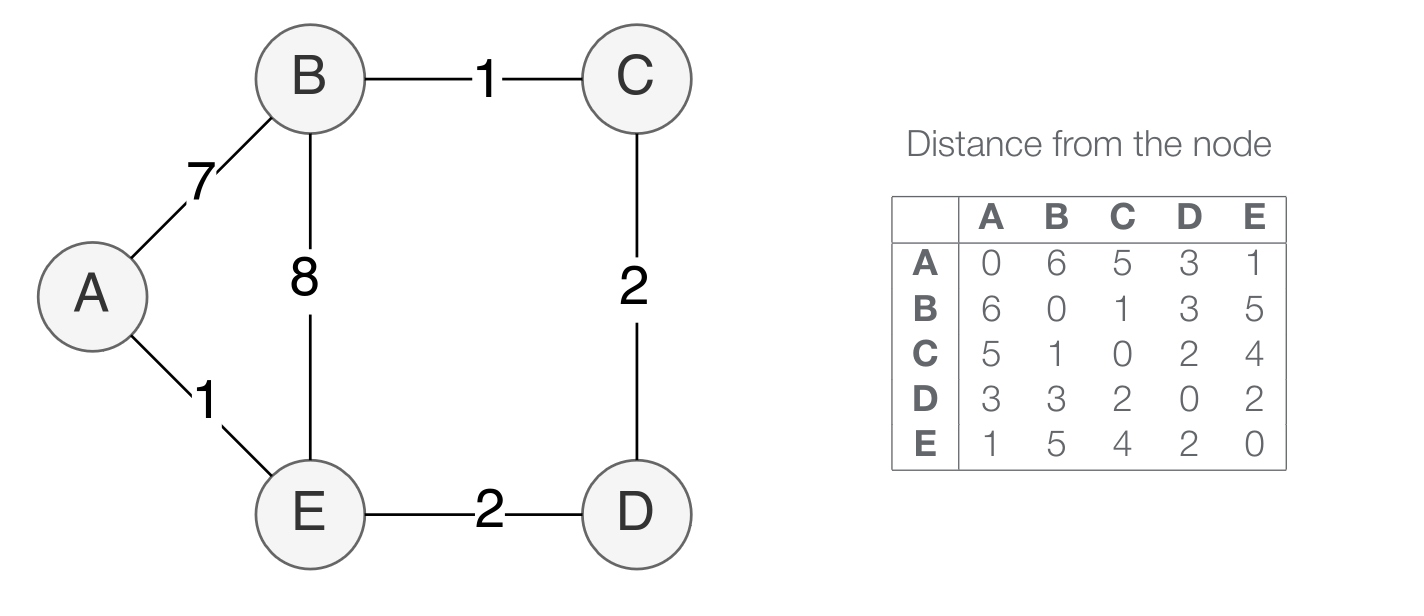
\includegraphics[width=0.7\linewidth]{Images/livello_ip/Bellman-Ford.png}
    \caption{Esempio di tabella di Routing con Bellman-Ford.}
\end{figure}

\subsection{Problemi}
Se il costo di un percorso aumenta e il percorso alternativo minimo contiene il percorso che è aumentato, il pacchetto non arriverà ma a destinazione ma farà avanti e indietro. Questo è chiamato \textbf{Rebound Effect}. Se un nodo è connesso tramite un collegamento e il collegamento si guasta, allora non si avrà stabilizzazione e si avrà un problema \textbf{Count-to-Infinity}.
\\
Le possibili soluzioni sono tre:
\begin{enumerate}
    \item Scegliere un \textbf{threeshold} per rappresentare il valore "infinito".
    \item \textbf{Split Horizon:} è necessario differenziare i vettori di distanza inviati ai nodi adiacenti. Il vettore di B inviato a C non conterrà le destinazioni raggiungibili tramite C.
    \item \textbf{Split Horizon with poisoned reverse:} se B raggiunge A passando per C, B avvertirà C che la sua distanza da A è infinita.
\end{enumerate}

\subsection{Algoritmi Link State}
Sono algoritmi \textbf{centralizzati}, necessitano di conoscere la \textbf{topologia} e il \textbf{costo} di ogni collegamento. Tutti i nodi hanno una visione identica e completa della rete e fanno diverse cose:
\begin{enumerate}
    \item Calcolano lo stato dei loro collegamenti.
    \item Trasmettono periodicamente l'identità e i costi dei loro collegamenti connessi.
    \item Calcolano i percorsi a costo minimo verso tutti gli altri nodi della rete utilizzando l'algoritmo di Dijkstra.
\end{enumerate}
Tutte queste informazioni sono contenute nel \textbf{Link State Packet}, nello specifico: 
\begin{itemize}
    \item Node ID.
    \item Lista dei vicini e costi dei collegamenti.
    \item Time To Live (TTL).
    \item Sequence Number per riconoscere eventuali errori.
\end{itemize}

\vspace*{0.02\textheight}
\textbf{PROPAGAZIONE DEI PACCHETTI:}
\begin{bashbox}
iif P is most recent packet form j then
    save P to database
    for all links != incoming link of P do
        Forward P
    else
        Discard P
\end{bashbox}

\subsubsection{Algortimo di Dijkstra}
Algoritmo iterativo, quindi, all'iterazione k, il nodo i conosce il percorso a costo minimo verso k nodi di destinazione. Abbiamo: 
\begin{itemize}
    \item $c(i, j)$ costo del collegamento tra il nodo \textbf{i} e il nodo \textbf{j}.
    \item $D(v)$ costo minimo del percorso verso il nodo \textbf{v} (minimo per l'iterazione corrente).
    \item $p(v)$ predecessore immediato di \textbf{v} lungo il percorso a costo minimo verso \textbf{v}.
    \item \textbf{N} gruppo di nodi il cui percorso a costo minimo è definitivamente noto.
\end{itemize}

\vspace*{0.01\textheight}
\textbf{INIZIALIZZAZIONE:}
\begin{bashbox}
NN = {u}
for all nodes v do
    if v is adjacent to u then
        D(v) = c(u, v)
    else
        D(v) = infinito
\end{bashbox}

\textbf{LOOP:}
\begin{bashbox}
rrepeat
    #Compute for all adjacent nodes i not in N the cost D(i)
    Add to N the node w with the minimum cost D(w)
    for all Nodes v adjacent to w and not in N do
        # new cost to v is the old one or the lowest cost to w plus the cost from w to v
        D(v) = min{D(v), D(w) + c(w, v)}
until all the nodes of the graph in N
\end{bashbox}

\begin{figure}[!htb]
    \centering
    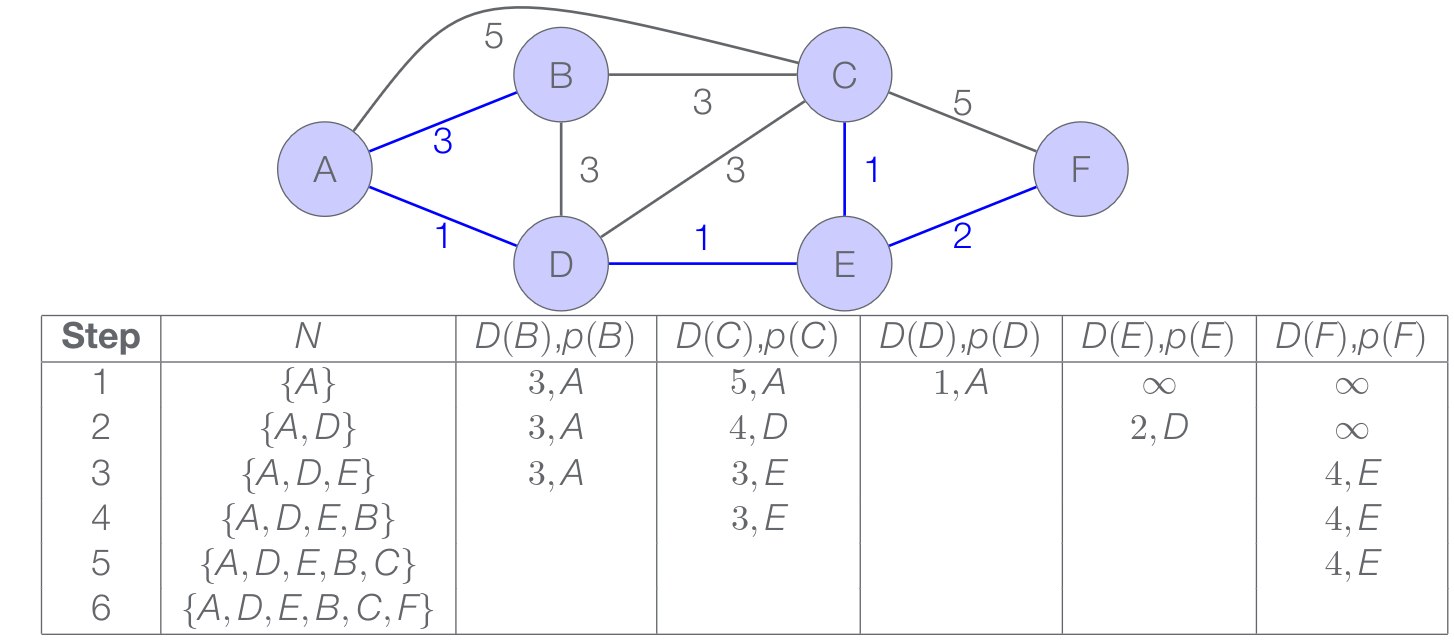
\includegraphics[width=0.8\linewidth]{Images/livello_ip/Dijkstra.png}
    \caption{Esempio di tabella di Routing con Dijkstra.}
\end{figure}

\subsection{Differenze fra Distan Vector Protocol e Algortimi Link State}
Non ci sono algoritmi migliori di altri, gli algortimi \textbf{Link State} sono usati spesso all'interno degli \textbf{AS}, invece, i \textbf{Distant Vector Algoritm} sono più usati fra \textbf{AS}.
\begin{center}
    \begin{minipage}{.45\linewidth}
        \begin{boxDef}
        \textbf{\textcolor{brown}{Distan Vector Protocol:}}
            \begin{itemize}
                \item Tutto ciò che è noto viene propagato solo ai vicini.
                \item Messaggi potenzialmente molto larghi.
                \item Numero di messaggi piccolo.
                \item Lenta convergenza e rischio di Rebound Effect o delay elevati.
                \item Requisiti di memoria piccoli.
                \item Calcoli del router basati su calcoli di altri router.
            \end{itemize}
        \end{boxDef}
    \end{minipage}
    \begin{minipage}{.45\linewidth}
        \begin{boxDef}
        \textbf{\textcolor{brown}{Algoritmi Link State:}}
            \begin{itemize}
                \item Le informazioni sono passate a tutti.
                \item Messaggi piccoli.
                \item Numero elevato di messaggi ($O(n)$ dove $n$ è il numero di nodi del grafo).
                \item Convergenza molto veloce.
                \item Requisiti di memoria elevati.
                \item Ogni router calcoli la route del percorso indipendentemente.
            \end{itemize}
        \end{boxDef}
    \end{minipage}
\end{center}

\newpage
\section{Routing a scala geografica}
Ogni \textbf{AS} ha un numero di identificazione, compreso tra 1 e 64511, assegnato da un'autorità di registrazione \textbf{Internet}. I numeri tra 64512 e 65535 sono riservati.
\\
Per il routing dentro gli AS (\textbf{Intra-AS routing}) si usa un \textbf{Interior Gateway Protocol}, cioè i router di un AS possono avere informazioni complete su tutti gli altri router dell'AS.
Per il routing fra AS (\textbf{Inter-AS routing}) si usa un \textbf{External Gateway Protocol}.
\\
Esistono diversi tipi di AS:
\begin{itemize}
    \item \textbf{Stub:} AS con una sola connessione a un altro AS.
    \item \textbf{Multi-Homed:} un AS è connesso con diversi altri AS, ma accetta solo traffico locale.
    \item \textbf{Transit:} un AS connesso a diversi AS che possono fungere da intermediari per l'AS a cui è connesso.
\end{itemize}
I protocolli di routing principali sono:
\begin{itemize}
    \item \textbf{Border Gateway Protocol (BGP)} per il routing \textbf{Inter-AS}.
    \item \textbf{Routing Information Protocol (RIP)} per il routing \textbf{Intra-AS}, come \textbf{Distance Vector Protocol}, non più usato.
    \item \textbf{Open Shortest Path First (OSPF)} per il routing \textbf{Intra-AS}, come \textbf{Link State Protocol}, quello che viene usato ora.
\end{itemize}

\subsection{Border Gateway Protocol (BGP)}
Protocollo delle backbones di Internet usato da ISP per gestire il traffico tra i sistemi autonomi in modo completamente decentralizzato. Ha alcune funzioni principali:
\begin{itemize}
    \item Scambio di informazioni di raggiungibilità tra AS vicini, chiamati \textbf{peer}.
    \item Propaga le informazioni di raggiungibilità a tutti i router all'interno di un AS con un meccanismo distribuito basato sull'algoritmo \textbf{Path Vector}.
    \item Determina i percorsi migliori in base alle informazioni di raggiungibilità e alle \textbf{politiche di instradamento}.
\end{itemize}
Per comunicare vengono utilizzate connessioni TCP semi-permanenti per consentire ai router vicini di comunicare, creando di fatto una \textbf{sessione} BGP. Le sessioni possono essere di due tipi: 
\begin{enumerate}
    \item \textbf{External session (E-BGP)} fra router (\textbf{Border Router)} di diversi AS.
    \item \textbf{Internal session (I-BGP} fra router (Transit Router) dello stesso AS.
\end{enumerate}

\begin{figure}[!htb]
    \centering
    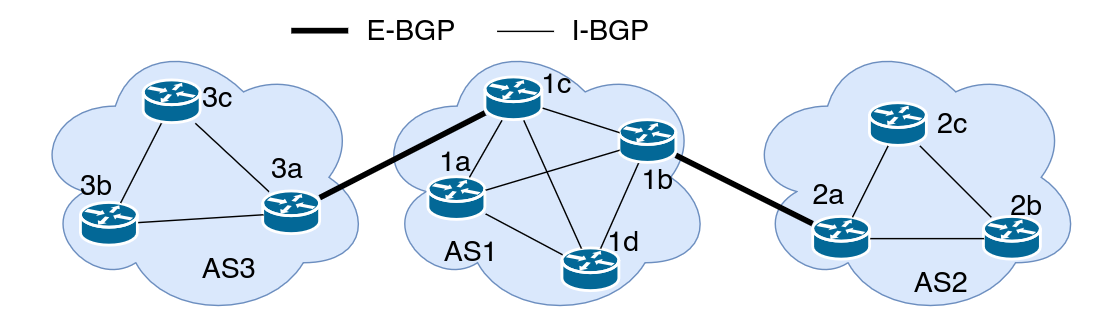
\includegraphics[width=0.8\linewidth]{Images/livello_ip/BGP.png}
    \caption{Routing BGP.}
\end{figure}

\subsubsection{Algoritmo Path Vector}
BGP utilizza Path Vector, una variante dell'algoritmo distribuito Distance Vector Protocol. Ogni aggiornamento di routing contiene non solo informazioni adiacenti, ma anche informazioni sull'intero percorso verso la destinazione tramite gli AS. Utilizza metriche e politiche locali nei processi decisionali e garantisce l'assenza di cicli.

\newpage
\subsection{Open Short Path First (OSPF)}
Il routing si basa sull'algoritmo centralizzato \textbf{Link State}. La topologia e costi noti a ciascun nodo, l'albero del percorso a costo minimo viene calcolato utilizzando l'algoritmo di \textbf{Dikstra} e memorizzato nel cosiddetto "database di stato dei collegamenti", distribuito a tutti i router periodicamente. Gli aggiornamenti, invece, vengono trasmessi in broadcast ai router dell'intero AS (\textbf{flooding}) direttamente su \textbf{IP}.
Le funzionalità principali sono: 
\begin{itemize}
    \item \textbf{Sicurezza:} autenticazione dei messaggi OSPF con algoritmi di crittografia.
    \item \textbf{Percorsi multipli con costo uguale:} possibilità di utilizzare percorsi multipli per instradare il traffico.
    \item \textbf{Supporto integrato per il routing unicast e multicast:} multicast OPSF (\textbf{MOSPF}) utilizza lo stesso database di collegamenti di OSPF.
    \item \textbf{Struttura gerarchica degli AS:} possibilità di strutturare grandi domini di routing in gerarchie di AS.
\end{itemize}

\subsection{Struttura di un messaggio OSPF}
Formato da un header in comune e un body che dipende dal tipo. \\
\begin{figure}[!htb]
    \centering
    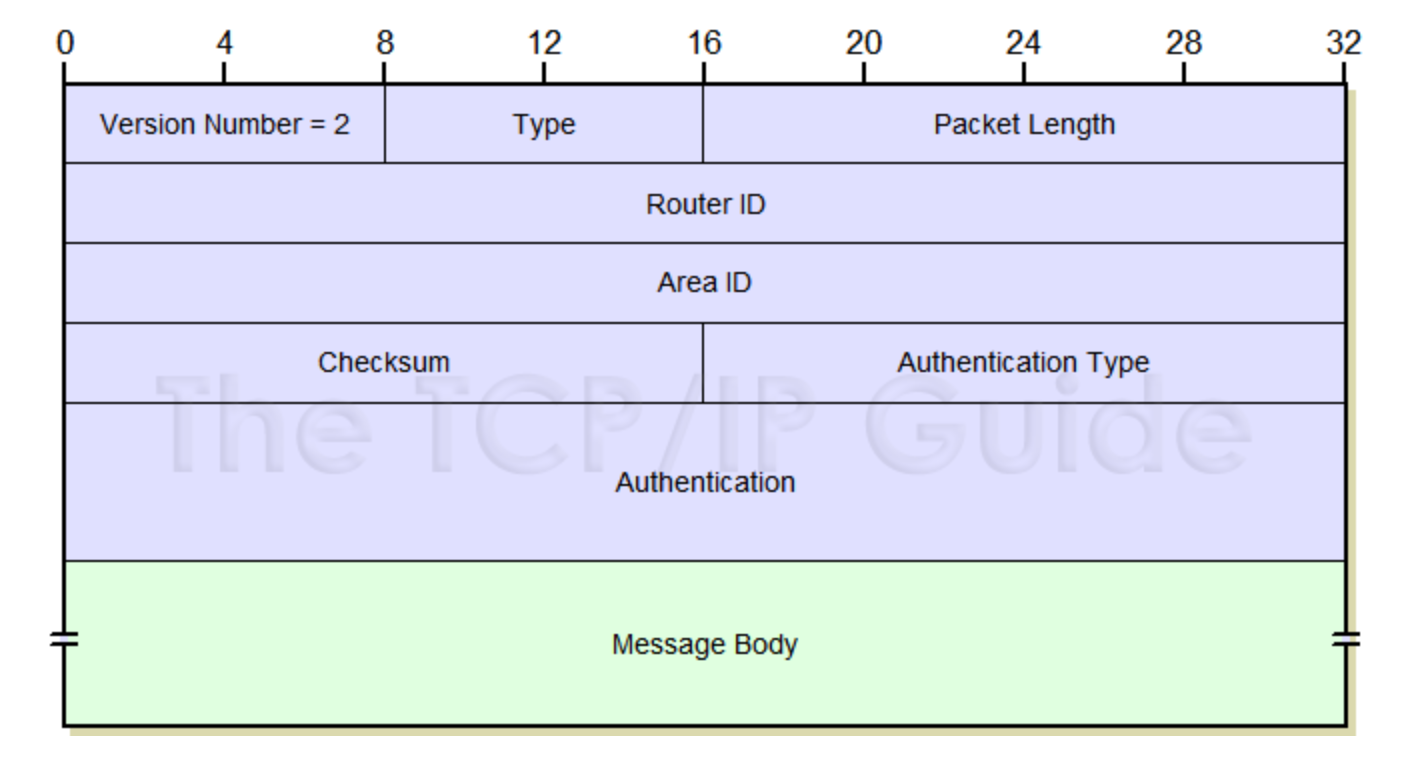
\includegraphics[width=0.70\linewidth]{Images/livello_ip/OSPF.png}
    \caption{Messaggio con OSPF.}
\end{figure}
L'header è formato da:
\begin{itemize}
    \item \textbf{Versione number.}
    \item \textbf{Tipo:}
    \begin{itemize}
        \item Hello.
        \item DB Description.
        \item Link State Req.
        \item Link State Update.
        \item Link State ACK.
    \end{itemize}
    \item \textbf{Dimensione:} misurata in byte (header + body).
    \item \textbf{Router ID:} ip dell'interfaccia da dove è inviato il messaggio.
    \item \textbf{AreaID:} area a cui il messaggio appartiene.
    \item \textbf{Checksum:} include tutto tranne che i campi di autenticazione.
    \item \textbf{Tipo di autenticazione:} può essere 0 (niente), 1 (con password) e 2 (crittografata).
    \item \textbf{Informazioni di autenticazione.}
\end{itemize}

\subsection{Struttura della gerarchia OSPF}
Consente di suddividere i grandi sistemi autonomi (AS) in aree in modo da avere una gerarchia interna a due livelli:
\begin{itemize}
    \item \textbf{Aree locali:} comunicano le rotte verso altre aree locali del sistema autonomo ai router di tali aree.
    \item \textbf{Aree Backbone:} instrada il traffico tra le aree del sistema autonomo, contiene tutti i border router.
\end{itemize} 
L'algoritmo Link State viene utilizzato all'interno di ciascuna area.

\section{IPv6}
